\question{13.5}{
    De weerstand van een blokje van een bepaalde metaalsoort hangt af van de temperatuur.
    Bij verschillende temperaturen ($X$) werd de weerstand ($Y$) gemeten.
    De resultaten zijn weergegeven in de volgende tabel:
    \begin{center}
        \begin{tabular}{cccccccc}
            \toprule
                {\bfseries Temperatuur (\si{\celsius})} & $-100$ & $-50$ & $0$ & $50$ & $100$ & $150$ & $200$ \\
            \cmidrule{1-1} \cmidrule{2-2} \cmidrule{3-3} \cmidrule{4-4} \cmidrule{5-5} \cmidrule{6-6} \cmidrule{7-7} \cmidrule{8-8}
                {\bfseries Weerstand (\si{\ohm})} & $13,2$ & $17,5$ & $21,3$ & $25,4$ & $28,9$ & $32,8$ & $36,8$ \\
            \bottomrule
        \end{tabular}
    \end{center}
}

\begin{enumerate}[label=(\alph*)]
    \item Ga ervan uit dat het verband tussen temperatuur en weerstand lineair is.
    Bepaal de regressielijn met de temperatuur als verklarende variabele.
    \answer{
        De regressielijn is van de vorm $Y = a + b\cdot X$, waarbij we de regressieco\"effici\"enten $a$ en $b$ bepalen aan de hand van 
        \begin{align*}
            b &= \frac{\overline{xy} - \overline{x} \cdot \overline{y}}{\overline{x^2} - (\overline{x})^2} \\
            a &= \overline{y} - b \cdot \overline{x}
        \end{align*}
        We moeten dus een tabel construeren met de gemiddelde $\overline{x}$, $\overline{y}$, $\overline{xy}$ en $\overline{x^2}$.
        \begin{center}
            \begin{tabular}{ccccc}
                \toprule
                    $x$ & $y$ & $xy$ & $x^2$ & $y^2$ \\
                \midrule
                    $-100$ & $13,2$ & $-1320$ & $10000$ & $174,24$ \\
                    $-50$ & $17,5$ & $-875$ & $2500$ & $306,25$ \\
                    $0$ & $21,3$ & $0$ & $0$ & $453,69$ \\
                    $50$ & $25,4$ & $1270$ & $2500$ & $645,16$ \\
                    $100$ & $28,9$ & $2890$ & $10000$ & $835,21$ \\
                    $150$ & $32,8$ & $4920$ & $22500$ & $1075,84$ \\
                    $200$ & $36,8$ & $7360$ & $40000$ & $1354,24$ \\
                \midrule
                    $\overline{x} = 50$ & $\overline{y} = 25,13$ & $\overline{xy} = 2035$ & $\overline{x^2} = 12500$ & $\overline{y^2} = 692,09$ \\
                \bottomrule
            \end{tabular}
        \end{center}

        We hebben nu alle grootheden die benodigd zijn om de co\"effici\"enten van de regressielijn $Y = a + b \cdot X$ te kunnen bepalen:
        \begin{align*}
            b   &= \frac{\overline{xy} - \overline{x} \cdot \overline{y}}{\overline{x^2} - (\overline{x})^2} \\
                &= \frac{2035 - 50 \cdot 25,1286}{12500 - 50^2} \\
                &= \frac{778,5714}{10000} \approx 0,0779 \\
            a   &= \overline{y} - b \cdot \overline{x} \\
                &= 25,1286 - 0,0779 \cdot 50 \\
                &\approx 21,2357.
        \end{align*}
        De formule van de regressielijn behorende bij deze steekproef is dus gelijk aan $Y = 21,2357+0,0779\cdot X$. 
        
        \begin{center}
            \resizebox{0.9\textwidth}{!}{
                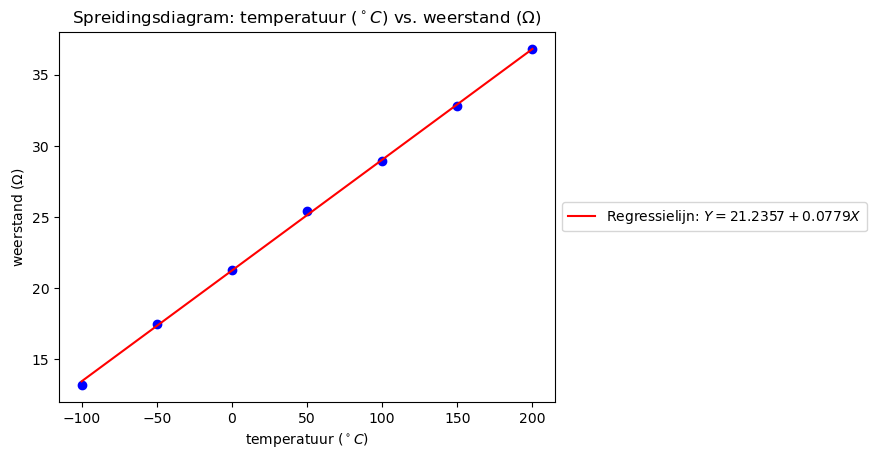
\includegraphics{opg13.5.png}
            }
        \end{center}
    }

    \item Welke weerstand kan men verwachten bij \SI{400}{\celsius}?
    \answer{
        De weerstand $Y$ die we verwachten bij een temperatuur $X$ vinden we door in te vullen in de regressielijn.
        Hieruit volgt dat bij een temperatuur van $X = $\SI{400}{\celsius} de verwachte weerstand gelijk is aan ongeveer $Y = 21,2357+0,0779 \cdot 400 \approx \SI{52.38}{\ohm}$.
        
        {
            \itshape Sidenote: we zijn in dit geval ver buiten de dataset aan het extrapoleren, want we hebben de regressielijn bepaald op basis van metingen voor temperaturen tussen \SI{-100}{\celsius} en \SI{200}{\celsius}.
            We moeten dus voorzichtig zijn met de aanname dat deze voorspelde waarde van de weerstand bij \SI{400}{\celsius} nauwkeurig zou zijn.
        }
    }

    \item Bij experimenten als het hier genoemde wordt de temperatuur vaak uitgedrukt in Kelvin (\si{\kelvin}).
    Hoe luidt de vergelijking van de regressielijn als de temperatuur in \si{\kelvin} wordt uitgedrukt?
    (Het nulpunt van de Kelvin-temperatuurschaal ligt bij \SI{-273}{\celsius}.
    Een stijging met \SI{1}{\celsius} is gelijk aan een stijging met \SI{1}{\kelvin}.)
    \answer{
        Zodra we de temperatuurschaal veranderen van Celsius (\si{\celsius}) naar Kelvin (\si{\kelvin}), moet bij iedere waarde van $X$ precies $273$ worden opgeteld.
        Laat nu $Z$ de temperatuur zijn in \si{\kelvin}.
        Dan geldt dus $Z = X + 273$, oftewel $X = Z - 273$.
        Invullen in de berekende regressielijn geeft:
        \begin{align*}
            Y   &= 21,2357 + 0,0779 \cdot (Z - 273) \\
                &= (21,2357 + 0,0779 \cdot -273) + 0,0779 \cdot Z \\
                &= -0,0310 + 0,0779 \cdot Z.
        \end{align*}  
        Deze lijn heeft dus exact dezelfde richtingsco\"effici\"ent (en is dus evenwijdig aan de regressielijn met de verklarende variabele $X$), maar heeft een lager gelegen snijpunt met de $Y$-as.
    }
\end{enumerate}